\section{Scientific Communication and the Flyspeck Project}\ednote{ESWC: Bascially, you shouldn't presume what you hope to prove. I think lots of your requirements and proposed solutions are very interesting, but they are independent of the realizing technology. In particular, I don't see the choice of using a wiki is any more significant that the choice to use Ruby or Python to implement the system. There was no experiment, as far as I could tell, with using arbitrary users, so there's little evidence that participants in the flyspeck project will find this  system so very useful. In particular, it's unclear to me that it will recruit significantly more participants.}
\label{sec:science-flyspeck}

\begin{wrapfigure}{r}{4.7cm}
  \centering
  \vspace{-1.0cm}
  \begin{tikzpicture}
    \node (s) at (0,0) {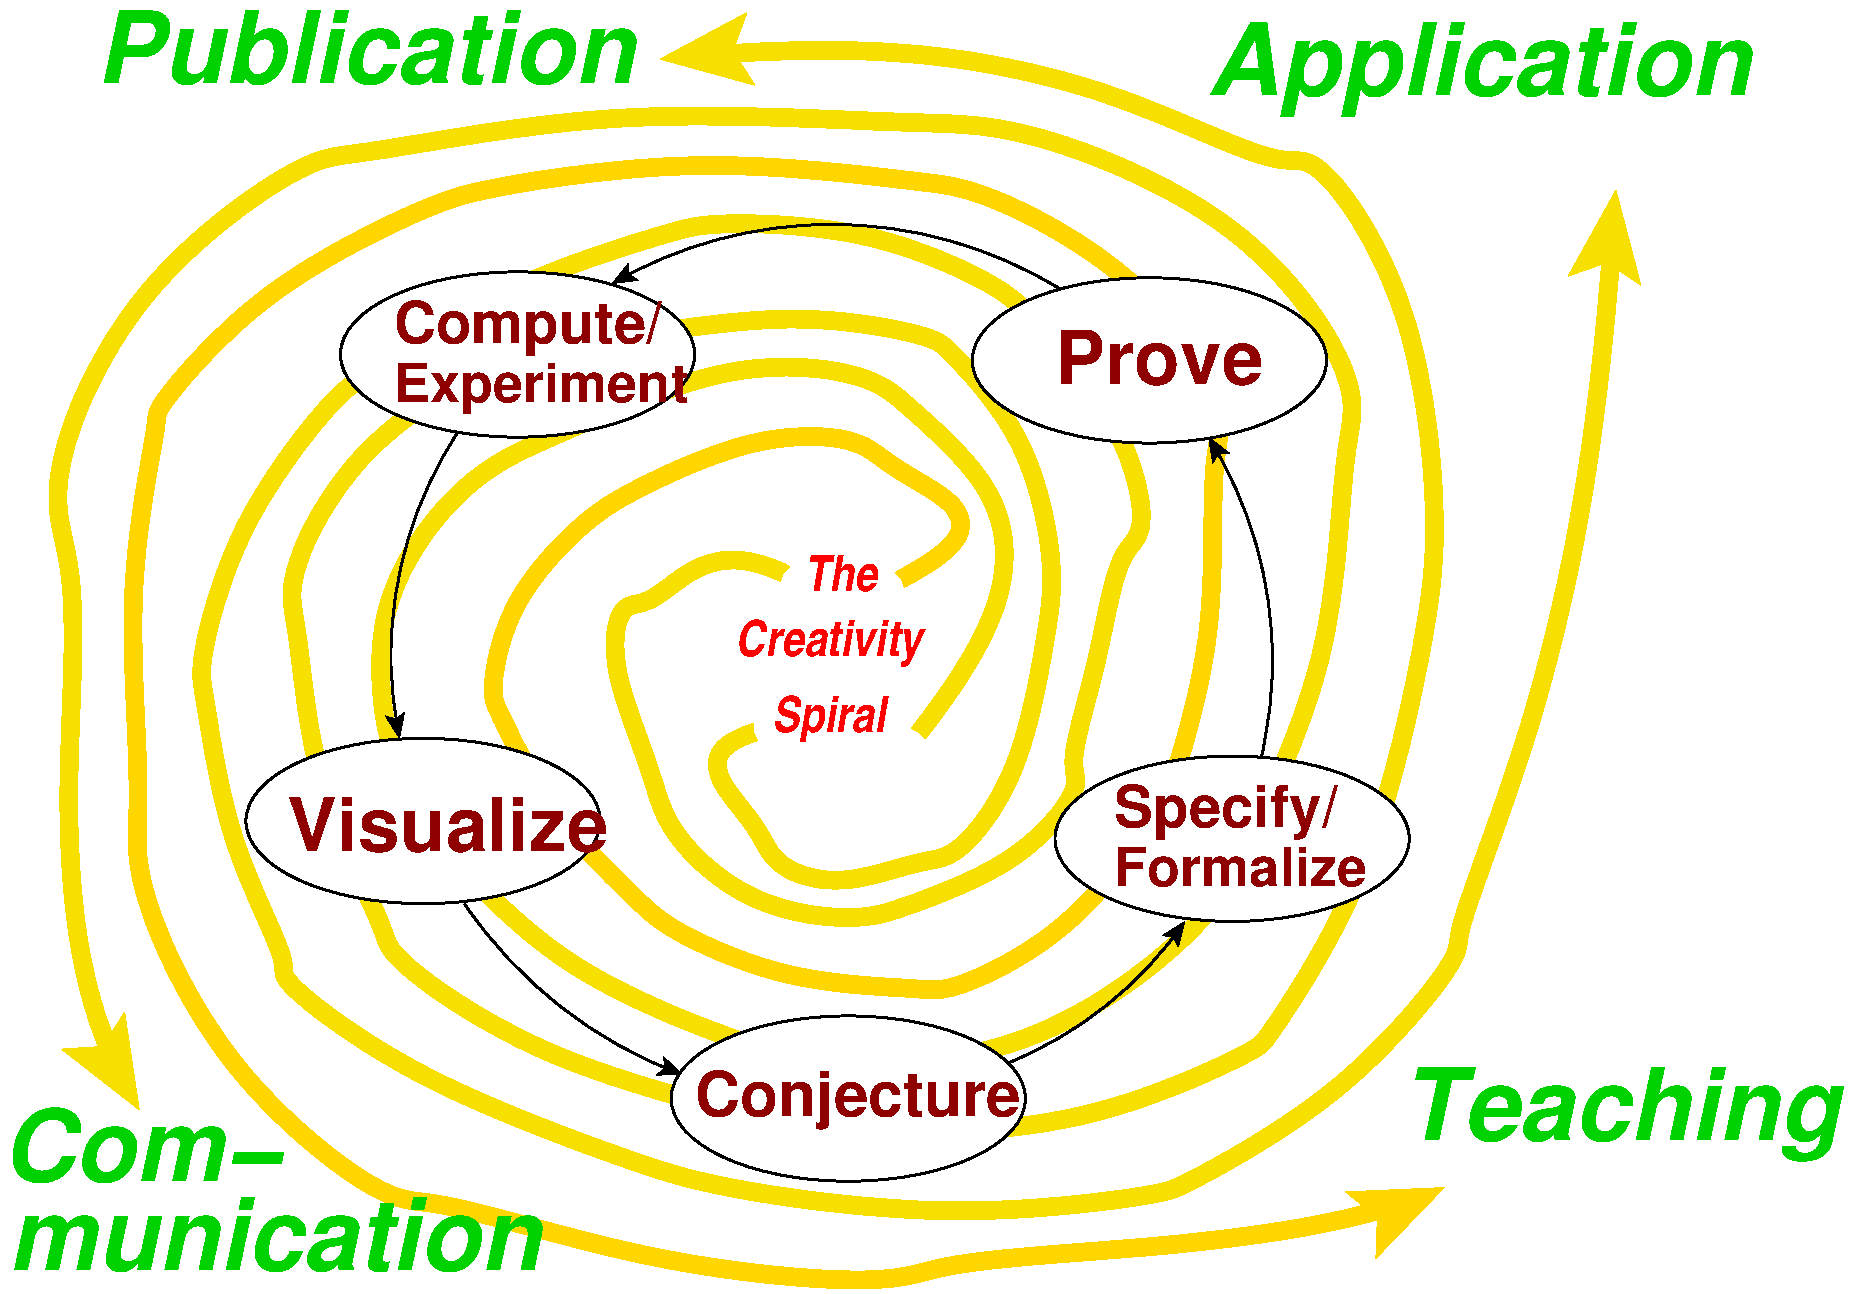
\includegraphics[width=4.5cm]{images/creativity-spiral}};
    \node at (s.south) {\scriptsize (B.\ Buchberger, 1995)};
  \end{tikzpicture}
  \vspace{-1.5cm}
\end{wrapfigure}
%% Documents are the most important medium in science.
%% , if we assume a broad definition of
%% ``document'', including any materialized item of (scientific) knowledge.  
%\begin{motivation}
\claim{Scientific communication consists mainly of exchanging documents, and a
%% : from informal drafts circulating inside a working group to published, well-structured books.
%% A
great deal of scientific work consists of collaboratively authoring them.}  Common instances are writing down first hypotheses, commenting on
results of experiments or project steps, and structuring, annotating, or
re-organizing existing items of knowledge, as depicted in Buchberger's figure on
the right.  \emph{Semantic markup languages} for
representing structures of scientific knowledge, and editing tools understanding
them, are a promising approach to supporting this work. %\end{motivation}
\begin{background}Besides generic approaches like SALT~\cite{Groza:SALT07}, the most extensive
work in semantic markup has been in the domain of mathematics.  Mathematical
logic, depending on symbols and relationships between symbols, naturally lends
itself well to formal exposition.
%% Mathematics has a ``long tradition in
%% the pursuit of conceptual clarity and representational
%% rigor''~\cite{Kohlhase:omdoc1.2}
%% \ednote{FR: this quote doesn't seem
%%   quote-worthy}  
Languages like MathML~\cite{CarlisleEd:MathML07},
OpenMath~\cite{BusCapCar:2oms04}, and OMDoc~\cite{Kohlhase:omdoc1.2} were
developed to represent the clearly defined and hierarchical structures of
mathematics in a way that preserves the intricate relationships.  OMDoc employs
Content MathML or OpenMath for structurally representing mathematical
\emph{objects} (symbols, numbers, equations, etc.) and adds two layers on top:
Objects or informal text can be annotated as mathematical \emph{statements}
(symbol declarations, definitions, axioms, theorems, proofs, examples, etc.),
and collections of interrelated statements can be grouped into \emph{theories}.\end{background}

\begin{background}With SWiM, a semantic wiki for mathematical knowledge
management~\cite{lange:swim-demo08}, we have investigated collaborative editing
of OMDoc documents.  Additionally, we host a public knowledge base and
experimental ground about mathematical knowledge management on the web, powered
by Semantic MediaWiki\footnote{\url{http://mathweb.org/wiki/}}.\end{background}  \claim{It has become
evident that a wiki is a suitable tool for supporting the workflow of
incremental formalization inherent to scientific writing.}  \claim{Wikis have not only
shown to be appropriate for \emph{writing}, but are also effective for project
management, e.\,g.\ in corporate settings~\cite{leuf01:wikiway,wikinomics}.}  We
are therefore interested in applying our technologies to scientific knowledge
engineering projects.

%%% Local Variables: 
%%% mode: latex
%%% TeX-master: "flyspeck-wiki-eswc08"
%%% End: 
